\documentclass[1p]{elsarticle_modified}
%\bibliographystyle{elsarticle-num}

%\usepackage[colorlinks]{hyperref}
%\usepackage{abbrmath_seonhwa} %\Abb, \Ascr, \Acal ,\Abf, \Afrak
\usepackage{amsfonts}
\usepackage{amssymb}
\usepackage{amsmath}
\usepackage{amsthm}
\usepackage{scalefnt}
\usepackage{amsbsy}
\usepackage{kotex}
\usepackage{caption}
\usepackage{subfig}
\usepackage{color}
\usepackage{graphicx}
\usepackage{xcolor} %% white, black, red, green, blue, cyan, magenta, yellow
\usepackage{float}
\usepackage{setspace}
\usepackage{hyperref}

\usepackage{tikz}
\usetikzlibrary{arrows}

\usepackage{multirow}
\usepackage{array} % fixed length table
\usepackage{hhline}

%%%%%%%%%%%%%%%%%%%%%
\makeatletter
\renewcommand*\env@matrix[1][\arraystretch]{%
	\edef\arraystretch{#1}%
	\hskip -\arraycolsep
	\let\@ifnextchar\new@ifnextchar
	\array{*\c@MaxMatrixCols c}}
\makeatother %https://tex.stackexchange.com/questions/14071/how-can-i-increase-the-line-spacing-in-a-matrix
%%%%%%%%%%%%%%%

\usepackage[normalem]{ulem}

\newcommand{\msout}[1]{\ifmmode\text{\sout{\ensuremath{#1}}}\else\sout{#1}\fi}
%SOURCE: \msout is \stkout macro in https://tex.stackexchange.com/questions/20609/strikeout-in-math-mode

\newcommand{\cancel}[1]{
	\ifmmode
	{\color{red}\msout{#1}}
	\else
	{\color{red}\sout{#1}}
	\fi
}

\newcommand{\add}[1]{
	{\color{blue}\uwave{#1}}
}

\newcommand{\replace}[2]{
	\ifmmode
	{\color{red}\msout{#1}}{\color{blue}\uwave{#2}}
	\else
	{\color{red}\sout{#1}}{\color{blue}\uwave{#2}}
	\fi
}

\newcommand{\Sol}{\mathcal{S}} %segment
\newcommand{\D}{D} %diagram
\newcommand{\A}{\mathcal{A}} %arc


%%%%%%%%%%%%%%%%%%%%%%%%%%%%%5 test

\def\sl{\operatorname{\textup{SL}}(2,\Cbb)}
\def\psl{\operatorname{\textup{PSL}}(2,\Cbb)}
\def\quan{\mkern 1mu \triangleright \mkern 1mu}

\theoremstyle{definition}
\newtheorem{thm}{Theorem}[section]
\newtheorem{prop}[thm]{Proposition}
\newtheorem{lem}[thm]{Lemma}
\newtheorem{ques}[thm]{Question}
\newtheorem{cor}[thm]{Corollary}
\newtheorem{defn}[thm]{Definition}
\newtheorem{exam}[thm]{Example}
\newtheorem{rmk}[thm]{Remark}
\newtheorem{alg}[thm]{Algorithm}

\newcommand{\I}{\sqrt{-1}}
\begin{document}

%\begin{frontmatter}
%
%\title{Boundary parabolic representations of knots up to 8 crossings}
%
%%% Group authors per affiliation:
%\author{Yunhi Cho} 
%\address{Department of Mathematics, University of Seoul, Seoul, Korea}
%\ead{yhcho@uos.ac.kr}
%
%
%\author{Seonhwa Kim} %\fnref{s_kim}}
%\address{Center for Geometry and Physics, Institute for Basic Science, Pohang, 37673, Korea}
%\ead{ryeona17@ibs.re.kr}
%
%\author{Hyuk Kim}
%\address{Department of Mathematical Sciences, Seoul National University, Seoul 08826, Korea}
%\ead{hyukkim@snu.ac.kr}
%
%\author{Seokbeom Yoon}
%\address{Department of Mathematical Sciences, Seoul National University, Seoul, 08826,  Korea}
%\ead{sbyoon15@snu.ac.kr}
%
%\begin{abstract}
%We find all boundary parabolic representation of knots up to 8 crossings.
%
%\end{abstract}
%\begin{keyword}
%    \MSC[2010] 57M25 
%\end{keyword}
%
%\end{frontmatter}

%\linenumbers
%\tableofcontents
%
\newcommand\colored[1]{\textcolor{white}{\rule[-0.35ex]{0.8em}{1.4ex}}\kern-0.8em\color{red} #1}%
%\newcommand\colored[1]{\textcolor{white}{ #1}\kern-2.17ex	\textcolor{white}{ #1}\kern-1.81ex	\textcolor{white}{ #1}\kern-2.15ex\color{red}#1	}

{\Large $\underline{11a_{260}~(K11a_{260})}$}

\setlength{\tabcolsep}{10pt}
\renewcommand{\arraystretch}{1.6}
\vspace{1cm}\begin{tabular}{m{100pt}>{\centering\arraybackslash}m{274pt}}
\multirow{5}{120pt}{
	\centering
	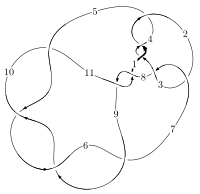
\includegraphics[width=112pt]{../../../GIT/diagram.site/Diagrams/png/509_11a_260.png}\\
\ \ \ A knot diagram\footnotemark}&
\allowdisplaybreaks
\textbf{Linearized knot diagam} \\
\cline{2-2}
 &
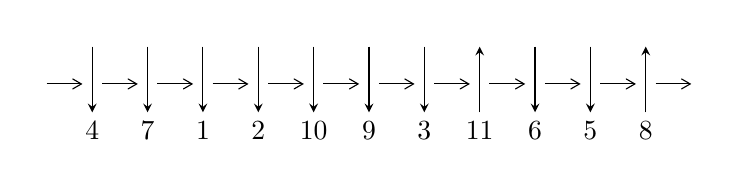
\begin{tikzpicture}[x=20pt, y=17pt]
	% nodes
	\node (C0) at (0, 0) {};
	\node (C1) at (1, 0) {};
	\node (C1U) at (1, +1) {};
	\node (C1D) at (1, -1) {4};

	\node (C2) at (2, 0) {};
	\node (C2U) at (2, +1) {};
	\node (C2D) at (2, -1) {7};

	\node (C3) at (3, 0) {};
	\node (C3U) at (3, +1) {};
	\node (C3D) at (3, -1) {1};

	\node (C4) at (4, 0) {};
	\node (C4U) at (4, +1) {};
	\node (C4D) at (4, -1) {2};

	\node (C5) at (5, 0) {};
	\node (C5U) at (5, +1) {};
	\node (C5D) at (5, -1) {10};

	\node (C6) at (6, 0) {};
	\node (C6U) at (6, +1) {};
	\node (C6D) at (6, -1) {9};

	\node (C7) at (7, 0) {};
	\node (C7U) at (7, +1) {};
	\node (C7D) at (7, -1) {3};

	\node (C8) at (8, 0) {};
	\node (C8U) at (8, +1) {};
	\node (C8D) at (8, -1) {11};

	\node (C9) at (9, 0) {};
	\node (C9U) at (9, +1) {};
	\node (C9D) at (9, -1) {6};

	\node (C10) at (10, 0) {};
	\node (C10U) at (10, +1) {};
	\node (C10D) at (10, -1) {5};

	\node (C11) at (11, 0) {};
	\node (C11U) at (11, +1) {};
	\node (C11D) at (11, -1) {8};
	\node (C12) at (12, 0) {};

	% arrows
	\draw[->,>={angle 60}]
	(C0) edge (C1) (C1) edge (C2) (C2) edge (C3) (C3) edge (C4) (C4) edge (C5) (C5) edge (C6) (C6) edge (C7) (C7) edge (C8) (C8) edge (C9) (C9) edge (C10) (C10) edge (C11) (C11) edge (C12) ;	\draw[->,>=stealth]
	(C1U) edge (C1D) (C2U) edge (C2D) (C3U) edge (C3D) (C4U) edge (C4D) (C5U) edge (C5D) (C6U) edge (C6D) (C7U) edge (C7D) (C8D) edge (C8U) (C9U) edge (C9D) (C10U) edge (C10D) (C11D) edge (C11U) ;
	\end{tikzpicture} \\
\hhline{~~} \\& 
\textbf{Solving Sequence} \\ \cline{2-2} 
 &
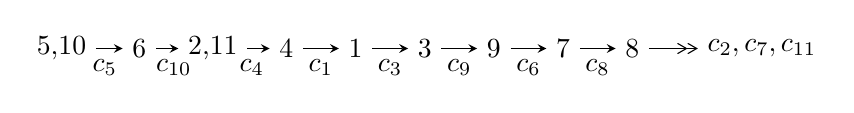
\begin{tikzpicture}[x=25pt, y=7pt]
	% node
	\node (A0) at (-1/8, 0) {5,10};
	\node (A1) at (1, 0) {6};
	\node (A2) at (33/16, 0) {2,11};
	\node (A3) at (25/8, 0) {4};
	\node (A4) at (33/8, 0) {1};
	\node (A5) at (41/8, 0) {3};
	\node (A6) at (49/8, 0) {9};
	\node (A7) at (57/8, 0) {7};
	\node (A8) at (65/8, 0) {8};
	\node (C1) at (1/2, -1) {$c_{5}$};
	\node (C2) at (3/2, -1) {$c_{10}$};
	\node (C3) at (21/8, -1) {$c_{4}$};
	\node (C4) at (29/8, -1) {$c_{1}$};
	\node (C5) at (37/8, -1) {$c_{3}$};
	\node (C6) at (45/8, -1) {$c_{9}$};
	\node (C7) at (53/8, -1) {$c_{6}$};
	\node (C8) at (61/8, -1) {$c_{8}$};
	\node (A9) at (10, 0) {$c_{2},c_{7},c_{11}$};

	% edge
	\draw[->,>=stealth]	
	(A0) edge (A1) (A1) edge (A2) (A2) edge (A3) (A3) edge (A4) (A4) edge (A5) (A5) edge (A6) (A6) edge (A7) (A7) edge (A8) ;
	\draw[->>,>={angle 60}]	
	(A8) edge (A9);
\end{tikzpicture} \\ 

\end{tabular} \\

\footnotetext{
The image of knot diagram is generated by the software ``\textbf{Draw programme}" developed by Andrew Bartholomew(\url{http://www.layer8.co.uk/maths/draw/index.htm\#Running-draw}), where we modified some parts for our purpose(\url{https://github.com/CATsTAILs/LinksPainter}).
}\phantom \\ \newline 
\centering \textbf{Ideals for irreducible components\footnotemark of $X_{\text{par}}$} 
 
\begin{align*}
I^u_{1}&=\langle 
u^{34}- u^{33}+\cdots+b+1,\;- u^{37}+2 u^{36}+\cdots+a-1,\;u^{38}-2 u^{37}+\cdots+u+1\rangle \\
I^u_{2}&=\langle 
b+1,\;- u^3+u^2+a-3 u+1,\;u^4- u^3+3 u^2-2 u+1\rangle \\
\\
\end{align*}
\raggedright * 2 irreducible components of $\dim_{\mathbb{C}}=0$, with total 42 representations.\\
\footnotetext{All coefficients of polynomials are rational numbers. But the coefficients are sometimes approximated in decimal forms when there is not enough margin.}
\newpage
\renewcommand{\arraystretch}{1}
\centering \section*{I. $I^u_{1}= \langle u^{34}- u^{33}+\cdots+b+1,\;- u^{37}+2 u^{36}+\cdots+a-1,\;u^{38}-2 u^{37}+\cdots+u+1 \rangle$}
\flushleft \textbf{(i) Arc colorings}\\
\begin{tabular}{m{7pt} m{180pt} m{7pt} m{180pt} }
\flushright $a_{5}=$&$\begin{pmatrix}1\\0\end{pmatrix}$ \\
\flushright $a_{10}=$&$\begin{pmatrix}0\\u\end{pmatrix}$ \\
\flushright $a_{6}=$&$\begin{pmatrix}1\\u^2\end{pmatrix}$ \\
\flushright $a_{2}=$&$\begin{pmatrix}u^{37}-2 u^{36}+\cdots+5 u+1\\- u^{34}+u^{33}+\cdots- u-1\end{pmatrix}$ \\
\flushright $a_{11}=$&$\begin{pmatrix}- u\\u\end{pmatrix}$ \\
\flushright $a_{4}=$&$\begin{pmatrix}u^{37}-2 u^{36}+\cdots+4 u+1\\- u^{34}+u^{33}+\cdots-2 u-1\end{pmatrix}$ \\
\flushright $a_{1}=$&$\begin{pmatrix}- u^9-4 u^7-3 u^5+2 u^3- u\\u^9+5 u^7+7 u^5+2 u^3+u\end{pmatrix}$ \\
\flushright $a_{3}=$&$\begin{pmatrix}u^{37}-2 u^{36}+\cdots+8 u^2+u\\- u^{35}- u^{34}+\cdots-2 u-1\end{pmatrix}$ \\
\flushright $a_{9}=$&$\begin{pmatrix}u\\u^3+u\end{pmatrix}$ \\
\flushright $a_{7}=$&$\begin{pmatrix}u^2+1\\u^4+2 u^2\end{pmatrix}$ \\
\flushright $a_{8}=$&$\begin{pmatrix}- u^5-2 u^3+u\\u^5+3 u^3+u\end{pmatrix}$\\ \flushright $a_{8}=$&$\begin{pmatrix}- u^5-2 u^3+u\\u^5+3 u^3+u\end{pmatrix}$\\&\end{tabular}
\flushleft \textbf{(ii) Obstruction class $= -1$}\\~\\
\flushleft \textbf{(iii) Cusp Shapes $= - u^{37}+2 u^{36}+\cdots+8 u-5$}\\~\\
\newpage\renewcommand{\arraystretch}{1}
\flushleft \textbf{(iv) u-Polynomials at the component}\newline \\
\begin{tabular}{m{50pt}|m{274pt}}
Crossings & \hspace{64pt}u-Polynomials at each crossing \\
\hline $$\begin{aligned}c_{1},c_{3},c_{4}\end{aligned}$$&$\begin{aligned}
&u^{38}-5 u^{37}+\cdots+3 u-1
\end{aligned}$\\
\hline $$\begin{aligned}c_{2},c_{7}\end{aligned}$$&$\begin{aligned}
&u^{38}- u^{37}+\cdots-8 u-16
\end{aligned}$\\
\hline $$\begin{aligned}c_{5},c_{6},c_{9}\\c_{10}\end{aligned}$$&$\begin{aligned}
&u^{38}-2 u^{37}+\cdots+u+1
\end{aligned}$\\
\hline $$\begin{aligned}c_{8},c_{11}\end{aligned}$$&$\begin{aligned}
&u^{38}+6 u^{37}+\cdots+93 u+19
\end{aligned}$\\
\hline
\end{tabular}\\~\\
\newpage\renewcommand{\arraystretch}{1}
\flushleft \textbf{(v) Riley Polynomials at the component}\newline \\
\begin{tabular}{m{50pt}|m{274pt}}
Crossings & \hspace{64pt}Riley Polynomials at each crossing \\
\hline $$\begin{aligned}c_{1},c_{3},c_{4}\end{aligned}$$&$\begin{aligned}
&y^{38}-39 y^{37}+\cdots-23 y+1
\end{aligned}$\\
\hline $$\begin{aligned}c_{2},c_{7}\end{aligned}$$&$\begin{aligned}
&y^{38}-27 y^{37}+\cdots-64 y+256
\end{aligned}$\\
\hline $$\begin{aligned}c_{5},c_{6},c_{9}\\c_{10}\end{aligned}$$&$\begin{aligned}
&y^{38}+42 y^{37}+\cdots+3 y+1
\end{aligned}$\\
\hline $$\begin{aligned}c_{8},c_{11}\end{aligned}$$&$\begin{aligned}
&y^{38}+30 y^{37}+\cdots-13361 y+361
\end{aligned}$\\
\hline
\end{tabular}\\~\\
\newpage\flushleft \textbf{(vi) Complex Volumes and Cusp Shapes}
$$\begin{array}{c|c|c}  
\text{Solutions to }I^u_{1}& \I (\text{vol} + \sqrt{-1}CS) & \text{Cusp shape}\\
 \hline 
\begin{aligned}
u &= -0.331390 + 0.800737 I \\
a &= -1.08027 + 1.42658 I \\
b &= \phantom{-}1.43349 - 0.08457 I\end{aligned}
 & -4.40003 + 3.17772 I & -9.24672 - 4.52124 I \\ \hline\begin{aligned}
u &= -0.331390 - 0.800737 I \\
a &= -1.08027 - 1.42658 I \\
b &= \phantom{-}1.43349 + 0.08457 I\end{aligned}
 & -4.40003 - 3.17772 I & -9.24672 + 4.52124 I \\ \hline\begin{aligned}
u &= \phantom{-}0.632534 + 0.587679 I \\
a &= \phantom{-}0.72801 - 2.04747 I \\
b &= \phantom{-}1.54993 + 0.28338 I\end{aligned}
 & -10.96810 - 8.77029 I & -12.03440 + 6.55590 I \\ \hline\begin{aligned}
u &= \phantom{-}0.632534 - 0.587679 I \\
a &= \phantom{-}0.72801 + 2.04747 I \\
b &= \phantom{-}1.54993 - 0.28338 I\end{aligned}
 & -10.96810 + 8.77029 I & -12.03440 - 6.55590 I \\ \hline\begin{aligned}
u &= \phantom{-}0.595823 + 0.532540 I \\
a &= -0.88414 + 1.11716 I \\
b &= -0.536492 - 0.820187 I\end{aligned}
 & -4.14241 - 4.72017 I & -10.42521 + 6.54233 I \\ \hline\begin{aligned}
u &= \phantom{-}0.595823 - 0.532540 I \\
a &= -0.88414 - 1.11716 I \\
b &= -0.536492 + 0.820187 I\end{aligned}
 & -4.14241 + 4.72017 I & -10.42521 - 6.54233 I \\ \hline\begin{aligned}
u &= -0.607436 + 0.495757 I \\
a &= -1.52782 - 1.27199 I \\
b &= -1.46016 + 0.02727 I\end{aligned}
 & -6.41754 + 2.06753 I & -11.71336 - 3.34688 I \\ \hline\begin{aligned}
u &= -0.607436 - 0.495757 I \\
a &= -1.52782 + 1.27199 I \\
b &= -1.46016 - 0.02727 I\end{aligned}
 & -6.41754 - 2.06753 I & -11.71336 + 3.34688 I \\ \hline\begin{aligned}
u &= \phantom{-}0.670848 + 0.404516 I \\
a &= \phantom{-}0.817417 - 0.255182 I \\
b &= \phantom{-}1.56238 - 0.24922 I\end{aligned}
 & -11.51120 + 4.37869 I & -13.39153 - 0.68267 I \\ \hline\begin{aligned}
u &= \phantom{-}0.670848 - 0.404516 I \\
a &= \phantom{-}0.817417 + 0.255182 I \\
b &= \phantom{-}1.56238 + 0.24922 I\end{aligned}
 & -11.51120 - 4.37869 I & -13.39153 + 0.68267 I\\
 \hline 
 \end{array}$$\newpage$$\begin{array}{c|c|c}  
\text{Solutions to }I^u_{1}& \I (\text{vol} + \sqrt{-1}CS) & \text{Cusp shape}\\
 \hline 
\begin{aligned}
u &= \phantom{-}0.603069 + 0.453875 I \\
a &= \phantom{-}0.323964 - 0.069070 I \\
b &= -0.604946 + 0.776470 I\end{aligned}
 & -4.37423 + 0.63202 I & -11.49824 + 0.19498 I \\ \hline\begin{aligned}
u &= \phantom{-}0.603069 - 0.453875 I \\
a &= \phantom{-}0.323964 + 0.069070 I \\
b &= -0.604946 - 0.776470 I\end{aligned}
 & -4.37423 - 0.63202 I & -11.49824 - 0.19498 I \\ \hline\begin{aligned}
u &= -0.458515 + 0.496866 I \\
a &= \phantom{-}0.735714 + 0.425841 I \\
b &= \phantom{-}0.295812 - 0.100934 I\end{aligned}
 & -0.58212 + 1.61412 I & -3.79024 - 4.58395 I \\ \hline\begin{aligned}
u &= -0.458515 - 0.496866 I \\
a &= \phantom{-}0.735714 - 0.425841 I \\
b &= \phantom{-}0.295812 + 0.100934 I\end{aligned}
 & -0.58212 - 1.61412 I & -3.79024 + 4.58395 I \\ \hline\begin{aligned}
u &= -0.166029 + 0.605237 I \\
a &= \phantom{-}0.54999 - 1.37311 I \\
b &= -0.197084 + 0.433714 I\end{aligned}
 & \phantom{-}0.92221 + 1.54825 I & -1.51822 - 6.63292 I \\ \hline\begin{aligned}
u &= -0.166029 - 0.605237 I \\
a &= \phantom{-}0.54999 + 1.37311 I \\
b &= -0.197084 - 0.433714 I\end{aligned}
 & \phantom{-}0.92221 - 1.54825 I & -1.51822 + 6.63292 I \\ \hline\begin{aligned}
u &= -0.599131\phantom{ +0.000000I} \\
a &= \phantom{-}0.814584\phantom{ +0.000000I} \\
b &= \phantom{-}1.47212\phantom{ +0.000000I}\end{aligned}
 & -6.92604\phantom{ +0.000000I} & -14.5410\phantom{ +0.000000I} \\ \hline\begin{aligned}
u &= \phantom{-}0.19248 + 1.43542 I \\
a &= -0.557197 - 0.105570 I \\
b &= \phantom{-}1.57803 - 0.19884 I\end{aligned}
 & -5.62113 + 1.29652 I & \phantom{-0.000000 } 0 \\ \hline\begin{aligned}
u &= \phantom{-}0.19248 - 1.43542 I \\
a &= -0.557197 + 0.105570 I \\
b &= \phantom{-}1.57803 + 0.19884 I\end{aligned}
 & -5.62113 - 1.29652 I & \phantom{-0.000000 } 0 \\ \hline\begin{aligned}
u &= \phantom{-}0.16452 + 1.49701 I \\
a &= \phantom{-}0.870156 - 0.798495 I \\
b &= -0.700266 + 0.746539 I\end{aligned}
 & \phantom{-}2.00271 - 2.06597 I & \phantom{-0.000000 } 0\\
 \hline 
 \end{array}$$\newpage$$\begin{array}{c|c|c}  
\text{Solutions to }I^u_{1}& \I (\text{vol} + \sqrt{-1}CS) & \text{Cusp shape}\\
 \hline 
\begin{aligned}
u &= \phantom{-}0.16452 - 1.49701 I \\
a &= \phantom{-}0.870156 + 0.798495 I \\
b &= -0.700266 - 0.746539 I\end{aligned}
 & \phantom{-}2.00271 + 2.06597 I & \phantom{-0.000000 } 0 \\ \hline\begin{aligned}
u &= \phantom{-}0.02138 + 1.51704 I \\
a &= \phantom{-}0.79272 + 1.61255 I \\
b &= -1.125240 - 0.315445 I\end{aligned}
 & \phantom{-}5.07701 - 1.17536 I & \phantom{-0.000000 } 0 \\ \hline\begin{aligned}
u &= \phantom{-}0.02138 - 1.51704 I \\
a &= \phantom{-}0.79272 - 1.61255 I \\
b &= -1.125240 + 0.315445 I\end{aligned}
 & \phantom{-}5.07701 + 1.17536 I & \phantom{-0.000000 } 0 \\ \hline\begin{aligned}
u &= -0.17777 + 1.51557 I \\
a &= -0.154126 - 1.301400 I \\
b &= -1.46693 + 0.08311 I\end{aligned}
 & \phantom{-}0.19906 + 4.87289 I & \phantom{-0.000000 } 0 \\ \hline\begin{aligned}
u &= -0.17777 - 1.51557 I \\
a &= -0.154126 + 1.301400 I \\
b &= -1.46693 - 0.08311 I\end{aligned}
 & \phantom{-}0.19906 - 4.87289 I & \phantom{-0.000000 } 0 \\ \hline\begin{aligned}
u &= -0.12286 + 1.53872 I \\
a &= \phantom{-}0.329499 + 0.682733 I \\
b &= \phantom{-}0.371714 - 0.234405 I\end{aligned}
 & \phantom{-}6.26465 + 3.65085 I & \phantom{-0.000000 } 0 \\ \hline\begin{aligned}
u &= -0.12286 - 1.53872 I \\
a &= \phantom{-}0.329499 - 0.682733 I \\
b &= \phantom{-}0.371714 + 0.234405 I\end{aligned}
 & \phantom{-}6.26465 - 3.65085 I & \phantom{-0.000000 } 0 \\ \hline\begin{aligned}
u &= \phantom{-}0.17843 + 1.53412 I \\
a &= -0.32146 + 1.73410 I \\
b &= -0.481260 - 0.864252 I\end{aligned}
 & \phantom{-}2.69845 - 7.51312 I & \phantom{-0.000000 } 0 \\ \hline\begin{aligned}
u &= \phantom{-}0.17843 - 1.53412 I \\
a &= -0.32146 - 1.73410 I \\
b &= -0.481260 + 0.864252 I\end{aligned}
 & \phantom{-}2.69845 + 7.51312 I & \phantom{-0.000000 } 0 \\ \hline\begin{aligned}
u &= -0.03636 + 1.55804 I \\
a &= \phantom{-}0.36918 - 1.51241 I \\
b &= -0.071818 + 0.599117 I\end{aligned}
 & \phantom{-}8.24732 + 2.22241 I & \phantom{-0.000000 } 0\\
 \hline 
 \end{array}$$\newpage$$\begin{array}{c|c|c}  
\text{Solutions to }I^u_{1}& \I (\text{vol} + \sqrt{-1}CS) & \text{Cusp shape}\\
 \hline 
\begin{aligned}
u &= -0.03636 - 1.55804 I \\
a &= \phantom{-}0.36918 + 1.51241 I \\
b &= -0.071818 - 0.599117 I\end{aligned}
 & \phantom{-}8.24732 - 2.22241 I & \phantom{-0.000000 } 0 \\ \hline\begin{aligned}
u &= \phantom{-}0.160891 + 0.403134 I \\
a &= -0.03733 + 2.61389 I \\
b &= -1.072260 - 0.128378 I\end{aligned}
 & -1.45280 - 0.68265 I & -5.04350 - 1.82049 I \\ \hline\begin{aligned}
u &= \phantom{-}0.160891 - 0.403134 I \\
a &= -0.03733 - 2.61389 I \\
b &= -1.072260 + 0.128378 I\end{aligned}
 & -1.45280 + 0.68265 I & -5.04350 + 1.82049 I \\ \hline\begin{aligned}
u &= \phantom{-}0.19856 + 1.55611 I \\
a &= -0.54782 - 2.02596 I \\
b &= \phantom{-}1.53547 + 0.31265 I\end{aligned}
 & -3.85806 - 11.81890 I & \phantom{-0.000000 } 0 \\ \hline\begin{aligned}
u &= \phantom{-}0.19856 - 1.55611 I \\
a &= -0.54782 + 2.02596 I \\
b &= \phantom{-}1.53547 - 0.31265 I\end{aligned}
 & -3.85806 + 11.81890 I & \phantom{-0.000000 } 0 \\ \hline\begin{aligned}
u &= -0.07622 + 1.60929 I \\
a &= -1.71521 + 1.01252 I \\
b &= \phantom{-}1.362500 - 0.126997 I\end{aligned}
 & \phantom{-}3.79825 + 4.60582 I & \phantom{-0.000000 } 0 \\ \hline\begin{aligned}
u &= -0.07622 - 1.60929 I \\
a &= -1.71521 - 1.01252 I \\
b &= \phantom{-}1.362500 + 0.126997 I\end{aligned}
 & \phantom{-}3.79825 - 4.60582 I & \phantom{-0.000000 } 0 \\ \hline\begin{aligned}
u &= -0.284804\phantom{ +0.000000I} \\
a &= \phantom{-}0.802881\phantom{ +0.000000I} \\
b &= -0.417854\phantom{ +0.000000I}\end{aligned}
 & -0.765706\phantom{ +0.000000I} & -13.9120\phantom{ +0.000000I}\\
 \hline 
 \end{array}$$\newpage\newpage\renewcommand{\arraystretch}{1}
\centering \section*{II. $I^u_{2}= \langle b+1,\;- u^3+u^2+a-3 u+1,\;u^4- u^3+3 u^2-2 u+1 \rangle$}
\flushleft \textbf{(i) Arc colorings}\\
\begin{tabular}{m{7pt} m{180pt} m{7pt} m{180pt} }
\flushright $a_{5}=$&$\begin{pmatrix}1\\0\end{pmatrix}$ \\
\flushright $a_{10}=$&$\begin{pmatrix}0\\u\end{pmatrix}$ \\
\flushright $a_{6}=$&$\begin{pmatrix}1\\u^2\end{pmatrix}$ \\
\flushright $a_{2}=$&$\begin{pmatrix}u^3- u^2+3 u-1\\-1\end{pmatrix}$ \\
\flushright $a_{11}=$&$\begin{pmatrix}- u\\u\end{pmatrix}$ \\
\flushright $a_{4}=$&$\begin{pmatrix}u^3- u^2+3 u\\-1\end{pmatrix}$ \\
\flushright $a_{1}=$&$\begin{pmatrix}-1\\0\end{pmatrix}$ \\
\flushright $a_{3}=$&$\begin{pmatrix}u^3- u^2+3 u-1\\-1\end{pmatrix}$ \\
\flushright $a_{9}=$&$\begin{pmatrix}u\\u^3+u\end{pmatrix}$ \\
\flushright $a_{7}=$&$\begin{pmatrix}u^2+1\\u^3- u^2+2 u-1\end{pmatrix}$ \\
\flushright $a_{8}=$&$\begin{pmatrix}u^2+1\\u^3- u^2+2 u-1\end{pmatrix}$\\ \flushright $a_{8}=$&$\begin{pmatrix}u^2+1\\u^3- u^2+2 u-1\end{pmatrix}$\\&\end{tabular}
\flushleft \textbf{(ii) Obstruction class $= 1$}\\~\\
\flushleft \textbf{(iii) Cusp Shapes $= 5 u^3-5 u^2+14 u-16$}\\~\\
\newpage\renewcommand{\arraystretch}{1}
\flushleft \textbf{(iv) u-Polynomials at the component}\newline \\
\begin{tabular}{m{50pt}|m{274pt}}
Crossings & \hspace{64pt}u-Polynomials at each crossing \\
\hline $$\begin{aligned}c_{1}\end{aligned}$$&$\begin{aligned}
&(u-1)^4
\end{aligned}$\\
\hline $$\begin{aligned}c_{2},c_{7}\end{aligned}$$&$\begin{aligned}
&u^4
\end{aligned}$\\
\hline $$\begin{aligned}c_{3},c_{4}\end{aligned}$$&$\begin{aligned}
&(u+1)^4
\end{aligned}$\\
\hline $$\begin{aligned}c_{5},c_{6}\end{aligned}$$&$\begin{aligned}
&u^4- u^3+3 u^2-2 u+1
\end{aligned}$\\
\hline $$\begin{aligned}c_{8}\end{aligned}$$&$\begin{aligned}
&u^4- u^3+u^2+1
\end{aligned}$\\
\hline $$\begin{aligned}c_{9},c_{10}\end{aligned}$$&$\begin{aligned}
&u^4+u^3+3 u^2+2 u+1
\end{aligned}$\\
\hline $$\begin{aligned}c_{11}\end{aligned}$$&$\begin{aligned}
&u^4+u^3+u^2+1
\end{aligned}$\\
\hline
\end{tabular}\\~\\
\newpage\renewcommand{\arraystretch}{1}
\flushleft \textbf{(v) Riley Polynomials at the component}\newline \\
\begin{tabular}{m{50pt}|m{274pt}}
Crossings & \hspace{64pt}Riley Polynomials at each crossing \\
\hline $$\begin{aligned}c_{1},c_{3},c_{4}\end{aligned}$$&$\begin{aligned}
&(y-1)^4
\end{aligned}$\\
\hline $$\begin{aligned}c_{2},c_{7}\end{aligned}$$&$\begin{aligned}
&y^4
\end{aligned}$\\
\hline $$\begin{aligned}c_{5},c_{6},c_{9}\\c_{10}\end{aligned}$$&$\begin{aligned}
&y^4+5 y^3+7 y^2+2 y+1
\end{aligned}$\\
\hline $$\begin{aligned}c_{8},c_{11}\end{aligned}$$&$\begin{aligned}
&y^4+y^3+3 y^2+2 y+1
\end{aligned}$\\
\hline
\end{tabular}\\~\\
\newpage\flushleft \textbf{(vi) Complex Volumes and Cusp Shapes}
$$\begin{array}{c|c|c}  
\text{Solutions to }I^u_{2}& \I (\text{vol} + \sqrt{-1}CS) & \text{Cusp shape}\\
 \hline 
\begin{aligned}
u &= \phantom{-}0.395123 + 0.506844 I \\
a &= \phantom{-}0.043315 + 1.227190 I \\
b &= -1.00000\phantom{ +0.000000I}\end{aligned}
 & -1.85594 - 1.41510 I & -11.17855 + 5.62908 I \\ \hline\begin{aligned}
u &= \phantom{-}0.395123 - 0.506844 I \\
a &= \phantom{-}0.043315 - 1.227190 I \\
b &= -1.00000\phantom{ +0.000000I}\end{aligned}
 & -1.85594 + 1.41510 I & -11.17855 - 5.62908 I \\ \hline\begin{aligned}
u &= \phantom{-}0.10488 + 1.55249 I \\
a &= \phantom{-}0.956685 + 0.641200 I \\
b &= -1.00000\phantom{ +0.000000I}\end{aligned}
 & \phantom{-}5.14581 - 3.16396 I & -6.32145 + 1.65351 I \\ \hline\begin{aligned}
u &= \phantom{-}0.10488 - 1.55249 I \\
a &= \phantom{-}0.956685 - 0.641200 I \\
b &= -1.00000\phantom{ +0.000000I}\end{aligned}
 & \phantom{-}5.14581 + 3.16396 I & -6.32145 - 1.65351 I\\
 \hline 
 \end{array}$$\newpage
\newpage\renewcommand{\arraystretch}{1}
\centering \section*{ III. u-Polynomials}
\begin{tabular}{m{50pt}|m{274pt}}
Crossings & \hspace{64pt}u-Polynomials at each crossing \\
\hline $$\begin{aligned}c_{1}\end{aligned}$$&$\begin{aligned}
&((u-1)^4)(u^{38}-5 u^{37}+\cdots+3 u-1)
\end{aligned}$\\
\hline $$\begin{aligned}c_{2},c_{7}\end{aligned}$$&$\begin{aligned}
&u^4(u^{38}- u^{37}+\cdots-8 u-16)
\end{aligned}$\\
\hline $$\begin{aligned}c_{3},c_{4}\end{aligned}$$&$\begin{aligned}
&((u+1)^4)(u^{38}-5 u^{37}+\cdots+3 u-1)
\end{aligned}$\\
\hline $$\begin{aligned}c_{5},c_{6}\end{aligned}$$&$\begin{aligned}
&(u^4- u^3+3 u^2-2 u+1)(u^{38}-2 u^{37}+\cdots+u+1)
\end{aligned}$\\
\hline $$\begin{aligned}c_{8}\end{aligned}$$&$\begin{aligned}
&(u^4- u^3+u^2+1)(u^{38}+6 u^{37}+\cdots+93 u+19)
\end{aligned}$\\
\hline $$\begin{aligned}c_{9},c_{10}\end{aligned}$$&$\begin{aligned}
&(u^4+u^3+3 u^2+2 u+1)(u^{38}-2 u^{37}+\cdots+u+1)
\end{aligned}$\\
\hline $$\begin{aligned}c_{11}\end{aligned}$$&$\begin{aligned}
&(u^4+u^3+u^2+1)(u^{38}+6 u^{37}+\cdots+93 u+19)
\end{aligned}$\\
\hline
\end{tabular}\newpage\renewcommand{\arraystretch}{1}
\centering \section*{ IV. Riley Polynomials}
\begin{tabular}{m{50pt}|m{274pt}}
Crossings & \hspace{64pt}Riley Polynomials at each crossing \\
\hline $$\begin{aligned}c_{1},c_{3},c_{4}\end{aligned}$$&$\begin{aligned}
&((y-1)^4)(y^{38}-39 y^{37}+\cdots-23 y+1)
\end{aligned}$\\
\hline $$\begin{aligned}c_{2},c_{7}\end{aligned}$$&$\begin{aligned}
&y^4(y^{38}-27 y^{37}+\cdots-64 y+256)
\end{aligned}$\\
\hline $$\begin{aligned}c_{5},c_{6},c_{9}\\c_{10}\end{aligned}$$&$\begin{aligned}
&(y^4+5 y^3+7 y^2+2 y+1)(y^{38}+42 y^{37}+\cdots+3 y+1)
\end{aligned}$\\
\hline $$\begin{aligned}c_{8},c_{11}\end{aligned}$$&$\begin{aligned}
&(y^4+y^3+3 y^2+2 y+1)(y^{38}+30 y^{37}+\cdots-13361 y+361)
\end{aligned}$\\
\hline
\end{tabular}
\vskip 2pc
\end{document}